% THIS IS SIGPROC-SP.TEX - VERSION 3.1
% WORKS WITH V3.2SP OF ACM_PROC_ARTICLE-SP.CLS
% APRIL 2009
%
% It is an example file showing how to use the 'acm_proc_article-sp.cls' V3.2SP
% LaTeX2e document class file for Conference Proceedings submissions.
% ----------------------------------------------------------------------------------------------------------------
% This .tex file (and associated .cls V3.2SP) *DOES NOT* produce:
%       1) The Permission Statement
%       2) The Conference (location) Info information
%       3) The Copyright Line with ACM data
%       4) Page numbering
% ---------------------------------------------------------------------------------------------------------------
% It is an example which *does* use the .bib file (from which the .bbl file
% is produced).
% REMEMBER HOWEVER: After having produced the .bbl file,
% and prior to final submission,
% you need to 'insert'  your .bbl file into your source .tex file so as to provide
% ONE 'self-contained' source file.
%
% Questions regarding SIGS should be sent to
% Adrienne Griscti ---> griscti@acm.org
%
% Questions/suggestions regarding the guidelines, .tex and .cls files, etc. to
% Gerald Murray ---> murray@hq.acm.org
%
% For tracking purposes - this is V3.1SP - APRIL 2009


\documentclass{acm_proc_article-sp}

\usepackage{comment}

% the natbib package allows both number and author-year (Harvard)
% style referencing;
%\usepackage{natbib}
%\usepackage{fancyhdr}
\usepackage[all]{xy}
\usepackage{rotating}
\usepackage{alltt}
%\usepackage{keywords}
\usepackage{keyval}
\usepackage{listings}
\usepackage{algorithm}
\usepackage{algorithmic}
%\usepackage{ifthen}
%\usepackage{lstmisc}
\usepackage{programs}
\usepackage{afterpage}
\usepackage{multirow}
\usepackage{array}

% if you use PostScript figures in your article
% use the graphics package for simple commands
 \usepackage{graphics}
% or use the graphicx package for more complicated commands
 \usepackage{graphicx}
% or use the epsfig package if you prefer to use the old commands
 %\usepackage{epsfig}

% The amssymb package provides various useful mathematical symbols
\usepackage{amssymb}

\def\CPP{C\raise.22ex\hbox{{\footnotesize +}}\raise.22ex\hbox{\footnotesize +}}
\def\BCPP{C\raise.22ex\hbox{{\footnotesize +}}\raise.22ex\hbox{\footnotesize +}}
\def\figline{\rule{\textwidth}{0.3mm}}
\def\shortline{\hrulefill}
\def\TURN#1{{\rotatebox{90}{~#1}}}



\begin{document}


% Languages
\def\CPP{C\raise.22ex\hbox{{\footnotesize +}}\raise.22ex\hbox{\footnotesize +}}
\def\CSHARP{C$^\#$}
\def\CPP{C\raise.22ex\hbox{{\footnotesize +}}\raise.22ex\hbox{\footnotesize +}}
\newcommand{\cpp}{C\raise.22ex\hbox{{\footnotesize +}}\raise.22ex\hbox{\footnotesize +}}

% File types
\def\tu{\tt tu}
\newcommand{\DrDobbs}{{Dr. Dobbs}}
\newcommand{\FTensor}{{FTensor}}
\newcommand{\layout}{{layout}}
\newcommand{\GPPDG}{{g++.dg}}
\newcommand{\netwerk}{{netwerk}}
\newcommand{\Pooma}{{POOMA}}
\newcommand{\GPP}{{GCC}}
\newcommand{\Bench}{\textsf{Benchmarks}}
\newcommand{\Libs}{\textsf{Libraries}}
\newcommand{\Apps}{\textsf{Applications}}
\newcommand{\gfour}{g$^4$re}
\newcommand{\Moz}{\textsf{Mozilla}}

\newcommand{\Blitz}{{Blitz\raise.22ex\hbox{{\footnotesize +}}\raise.22ex\hbox{\footnotesize +}}}
\newcommand{\gpp}{g\raise.22ex\hbox{{\footnotesize +}}\raise.22ex\hbox{\footnotesize +}}
\newcommand{\JPP}{J\raise.22ex\hbox{{\footnotesize +}}\raise.22ex\hbox{\footnotesize +}}

\def\GCC{\sf GCC}
\def\Fluxbox{\sf {Fluxbox}}
\def\Doxygen{\sf Doxygen}
\def\FiSim{\sf FiSim}
\def\Necko{\sf Necko}
\def\Gecko{\sf Gecko}
\def\XPCOM{\sf XPCOM}
\def\Mozilla{\sf Mozilla}

\def\figline{\rule{\textwidth}{0.3mm}}
\def\shortline{\hrulefill}
\def\TURN#1{{\rotatebox{90}{~#1}}}

\newcommand{\Ar}{\mathbf{A_r}}
\newcommand{\Ac}{\mathbf{A_c}}
\newcommand{\A}{\mathbf{A}}
\newcommand{\R}{\mathbf{R}}
\renewcommand\arraystretch{1.3}

\newcommand{\insertgraphic}[4]
% {~}
  {\begin{center}
  \scalebox{#2}[#2]{\includegraphics{#1}}
  \parbox{5.5in}{\caption{\small #4 \label{#3}}}\end{center}}
% \insertgraphic{file}{scalefactor}{label}{captiontext}


% Applications/Libraries
\def\CPPX{\em CPPX}
\def\Columbus{\em Columbus}
\def\Datrix{\em Datrix}
\def\GCCXML{\em GCC.XML}
\def\SourceNavigator{\em Source--Navigator}
\def\TUAnalyzer{\em TUAnalyzer}
\def\XOGASTAN{\em XOGASTAN}
\def\bison{\em bison}
\def\dot{\em dot}
\def\gcc{\em gcc}
\def\gxlvalidator{\em gxlvalidator}
\def\gzip{\em gzip}
\def\expat{\em expat}
\def\flex{\em flex}
\def\xsltproc{\em xsltproc}
\def\zlib{\em zlib}
\def\ld{\em ld}
\def\pulse{\em pulse}

% Test suite
\def\AvP{\em {AvP}}
\def\CppUnit{\em {CppUnit}}
\def\Doxygen{\em Doxygen}
\def\FluxBox{\em {FluxBox}}
\def\FOX{\em {FOX}}
\def\HippoDraw{\em {HippoDraw}}
\def\Jikes{\em Jikes}
\def\Keystone{\em Keystone}
\def\Licq{\em Licq}
\def\Pixie{\em Pixie}
\def\Scintilla{\em Scintilla}
\def\Scribus{\em Scribus}

\def\ASC{\em {ASC}}
\def\Freespace{\em Freespace2}
\def\Scorched{\em Scorched3D}

% Schemas
\def\CPPINFO{\sf CppInfo}
\def\GENERIC{\sc generic}
\def\CCFG{\sf CCFG}
\def\CDG{\sf CDG}
\def\CFG{\sf CFG}
\def\CallGraph{\sf Call Graph}
\def\ClassDiagram{\sf Class Diagram}
\def\ClassFirewall{\sf Class Firewall}
\def\ICFG{\sf ICFG}
\def\ORD{\sf ORD}
\def\PDG{\sf PDG}
\def\SDG{\sf SDG}

% g4re
\def\gfourre{\sf g$^4$re}
\def\GXLSW{\sf GxlSW}
\def\gfourrepackage{\sf g4re}
\def\gfourxformer{\sf g4xformer}
\def\generic{\sf generic}
\def\cppinfo{\sf cppinfo}
\def\schema{\sf schema}
\def\serialization{\sf serialization}
\def\linker{\sf Linker}
\def\api{\sf api}

\def\builder{\sf builder}
\def\ctd{\sf ctd}
\def\visualizer{\sf visualizer}

\newcommand{\hilight}[1]{\colorbox{yellow}{#1}}



\title{Design and Implementation of a \\
Language-Complete {\CPP} Semantic Graph
\permission{Permission to make digital or hard copies of all or part 
of this work for personal or classroom use is granted without fee 
provided that copies are not made or distributed for profit or commercial 
advantage and that copies bear this notice and the full citation on the 
first page. To copy otherwise, or republish, to post on servers or to 
redistribute to lists, requires prior specific permission and/or a fee.
ACMSE'12, March 29–31, 2012, Tuscaloosa, AL, USA.
Copyright 2012 ACM 978-1-4503-1203-5/12/03...\$10.00.}
}

\numberofauthors{1} 
\author{
\alignauthor
Edward B. Duffy and Brian A. Malloy \\
       \affaddr{School of Computing}\\
       \affaddr{Clemson University}\\
       \affaddr{Clemson, SC 29634, USA}\\
       \email{\{eduffy,malloy\}@cs.clemson.edu}
}


\maketitle
%------------------------------------------------------------------------- 
% take the % away on next line to produce the final camera-ready version 
\thispagestyle{empty}

\begin{abstract}


In this paper, we describe a system, Hylian, for construction
of a language-complete
abstract semantic graph that can be used for statement-level
analysis, both static and dynamic, of a {\CPP} application.
We begin by extending the GNU $gcc$ parser to generate parse 
trees in XML format for each of the compilation units in a {\CPP} 
application.  We then provide verification that the generated parse 
trees are structurally equivalent to the code in the original {\CPP} 
application.
We use the generated parse trees, together with an augmented version of
the {\em gcc} test suite,
to recover a grammar for the {\CPP} dialect that we parse.
%We use the recovered grammar to generate a schema for
%further verification of the parse trees and evaluate the coverage 
%provided by our {\CPP} test suite.
We then construct the Abstract Semantic Graph, ASG, by extending the 
parse tree for each compilation unit with semantic 
information derived from the parse trees and guided by the {\CPP} 
language standard.
Finally, we link the ASGs for all of the compilation units into a 
unified ASG for the entire application under study. 

\end{abstract}

\section{Introduction}
\label{sec:intro}


The software maintenance process, including comprehension, modification,
and refactoring of complex multi-par\-a\-digm systems, requires 
extensive and detailed information about the system under study.
However, software artifacts that provide this information are
frequently unavailable and for large, open-source applications,
they are virtually nonexistent.
Thus, much of the research in software maintenance has focused 
on the development of inquiry and analysis tools to automate the
process of generating information to improve comprehension, and to 
facilitate analysis, modification and testing of the application under 
study.

However, the {\CPP} language has proven to be particularly problematic 
for maintenance engineers interested in developing tools to facilitate
analysis and modification of {\CPP} applications.
The difficulty in developing tools for {\CPP} is mostly 
due to the scope and complexity of the language; for example,
the grammatical representation of {\CPP} has been shown to be  
larger and more complex than other, commonly used
languages \cite{Power-Malloy:04}.
A particularly perplexing problem for {\CPP} maintenance engineers
 entails the correct recognition of the language constructs
as specified in the ISO standard, for example class template partial
specializations and argument-dependent lookup \cite[\S A.8]{C++standard98}.
Moreover, statement-level information,
which is required for pointer analysis and program 
slicing \cite{binkley2006,gallagher2003,Harrold1996MAY,Weiser84},
relies on the correct recognition of expressions such
as {\em expression}, {\em postfix-expression},
and {\em unary-expression} \cite[\S A.4]{C++standard98}.

Nevertheless, the {\CPP} language is frequently used and recently
has been shown to outperform other, commonly used, languages
by a large margin \cite{preez2011}.
Therefore, to support software maintenance and other software
engineering efforts for the {\CPP} language, it's important to
develop analysis tools for the language.
Several research projects have attempted to address the problem
of providing analysis of {\CPP} language constructs, including
Elkhound, {\sf SourceNavigator}\texttrademark, {\sf Columbus},
{\gfourre}, and libclang 
\cite{elsa2007,sourcenav,columbus2005,kraft05-wcre,kraft06-ist,www-libclang}.
However, due to the difficulties in parsing the {\CPP} language,
these projects are unable to provide statement level analysis.
Therefore, they are unable to regenerate the source code, which
precludes dynamic analysis, and they cannot provide details
about statements and expressions, which precludes analysis such
as pointer alias and slicing.

In this paper, we describe our extension of a system, Hylian,
which utilizes the {\em gcc} parser to provide statement level
analysis of {\CPP} programs. The initial phases of Hylian were 
described in references 
\cite{duffy05-sera,duffy-wcre07,Duffy-Malloy:2007,Duffy-etal:2008,IJSEKE}.
In this paper, we describe our construction of an abstract semantic 
graph (ASG), that is {\em language-complete}, which is a semantic graph
that includes all aspects defined in the language standard.
Our focus is an ASG that is language-complete
for the 2003 revised ISO {\CPP} language standard; our current
implementation does not include the {\CPP}11 standard, recently
ratified \cite{isocpp-11}.
A semantic graph that completely defines {\CPP} must include:
evaluation and lookup
of constants, full type resolution for names, determination of
type equivalency and type promotion, full and partial template
instantiation, operator overload resolution, function and method
resolution including argument dependent name lookup, implicit
method invocation commonly used in class construction and destruction.
The current implementation of Hylian provides information about
all of these constructs.

In the next section, we review projects that relate to
our work, and in Section \ref{sec:overview} we provide an overview 
of the three phases of Hylian. In Section \ref{sec:method} we 
provide details about construction of the Hylian ASG, and
in Section \ref{sec:results} we list statistics that 
summarize efficiency considerations for ASG construction, including 
some size results for an ASG for a popular video game. 
In Section \ref{sec:conclude} we draw conclusions.




\section{Related Work}
\label{sec:related}

In this section, we review the research that facilitates static or 
dynamic analysis of {\CPP} language constructs, from high level
constructs such as classes and class hierarchies, to low level
constructs, such as statements or expressions.
Statement and expression analysis requires a parser front-end that
is language complete for the ISO standard, and can syntactically
and semantically represent all constructs in the language. 
%In the case of the {\CPP} language, these constructs include
%full type resolution for names, determination of
%type equivalency and type promotion, full and partial template
%instantiation, operator overload resolution, function and method
%resolution including argument dependent name lookup, and implicit
%method invocation commonly used in class construction and destruction.

We only review the work with a focus on analysis of {\CPP}
programs, and that make this analysis information available to
a developer, typically in graph form.
For example, Elkhound is a parser generator that uses the Generalized 
LR (GLR) parsing algorithm \cite{elsa2007,tomita85,vandenbrand98}.
The Elkhound parser, Elsa, attempts to accommodate several dialects 
of {\CPP} including {\em gcc} and Visual {\CPP} \cite{elsa2007}.
Elsa can accommodate most of the {\CPP} grammar,
but does not fully accommodate either dialect.
For example, only 89\% of the test cases in the {\em gcc} test suite, 
were parsed by Elsa. However, for {\Fluxbox}, a lightweight
window manager for X, only 32 of the 74 translation units were 
parsed by Elsa \cite{www-fluxbox}.  Also, the Elsa project has 
not been recently updated \cite{elsa2007}.
By contrast, Hylian can parse all test cases in the {\em gcc} test
suite and we have been able to provide analysis of the {\Fluxbox}
application \cite{kraft-tse}. 
To make the analysis information available, Hylian
builds an abstract semantic graph (ASG) with subgraphs for all
{\CPP} language constructs, including instantiation of templates.

{\sf SourceNavigator}\texttrademark is an analysis and graphical 
framework from Red Hat \cite{sourcenav}. SourceNavigator 
accepts C, {\CPP}, Java, Tcl, FORTRAN, and COBOL, and the 
accompanying fuzzy parser extracts enough high level information to 
provide class hierarchies, imprecise call graphs, and include graphs.
However, since {\sf SourceNavigator} employs a fuzzy parse, it
does not provide statement level information.

{\sf Columbus} is an integrated reverse engineering framework 
supporting fact extraction, linking, and analysis for C and {\CPP} 
programs \cite{columbus2005}. 
{\sf Columbus} provides output in a variety of formats, including
{CPPML} (OCaml-like pattern-matching extensions for {\CPP}),
{GXL} (a schema for storing graphs in XML), {RSF} (a reverse-engineering
tool that supports source code transformations for {\CPP} applications),
and {XMI} (an Object Manager Group metadata standard for XML).
Nevertheless, {\sf Columbus} is unable to fully accept templates,
as noted in reference \cite{tuanalyzer04}.


The {\gfourre} system, like Hylian, uses {\em gcc} as its parser
front-end. {\gfourre} is designed as a tool chain, and consists 
of applications and libraries that can be used either individually 
or as a single unit \cite{kraft05-wcre,kraft06-ist}.
The implementation of {\gfourre} uses  a GXL-based pipe-filter 
architecture, including a set of loosely coupled, reusable 
modules including an {\em ASG module}.
Advantages of {\gfourre} include an API to provide easy access to
information about declarations, including classes, functions,
and variables, as well as information about scopes, types, and
control statements. 
However, {\gfourre} is not code-complete, so that 
the original source code cannot be regenerated from
the {\em ASG module}. 
Thus, the {\gfourre} system is limited to static analysis of
type information and cannot provide information about statements
or expressions.

An alternative, open source library for parsing {\CPP} language
constructs includes clang \cite{www-clang}, and its C interface, 
libclang \cite{www-libclang};
Thus, clang is the parser front-end used by libclang; 
the goal of libclang is to facilitate IDE development,
most notably, Apple's XCode.  The libclang API can
track variable declarations, provide syntax highlighting, code 
completion, symbol renaming, and cross-referencing, including 
references to global variables across compilation units. 
However, even though information about statements is complete in
clang, libclang does not present all of this information
to clients of the API.
However, like libclang and {\em gcc}, this information is not 
readily available, so that an interested developer
must investigate clang internals, whose documentation exists in 
the form of source code comments and developer mailing lists.
Thus, the complete information about statements known to clang
is not accessible to a libclang user, either in graph form, or as
an easily accessible API.



\section{Overview of The System}
\label{sec:overview}


\begin{figure*}[t]
\centerline{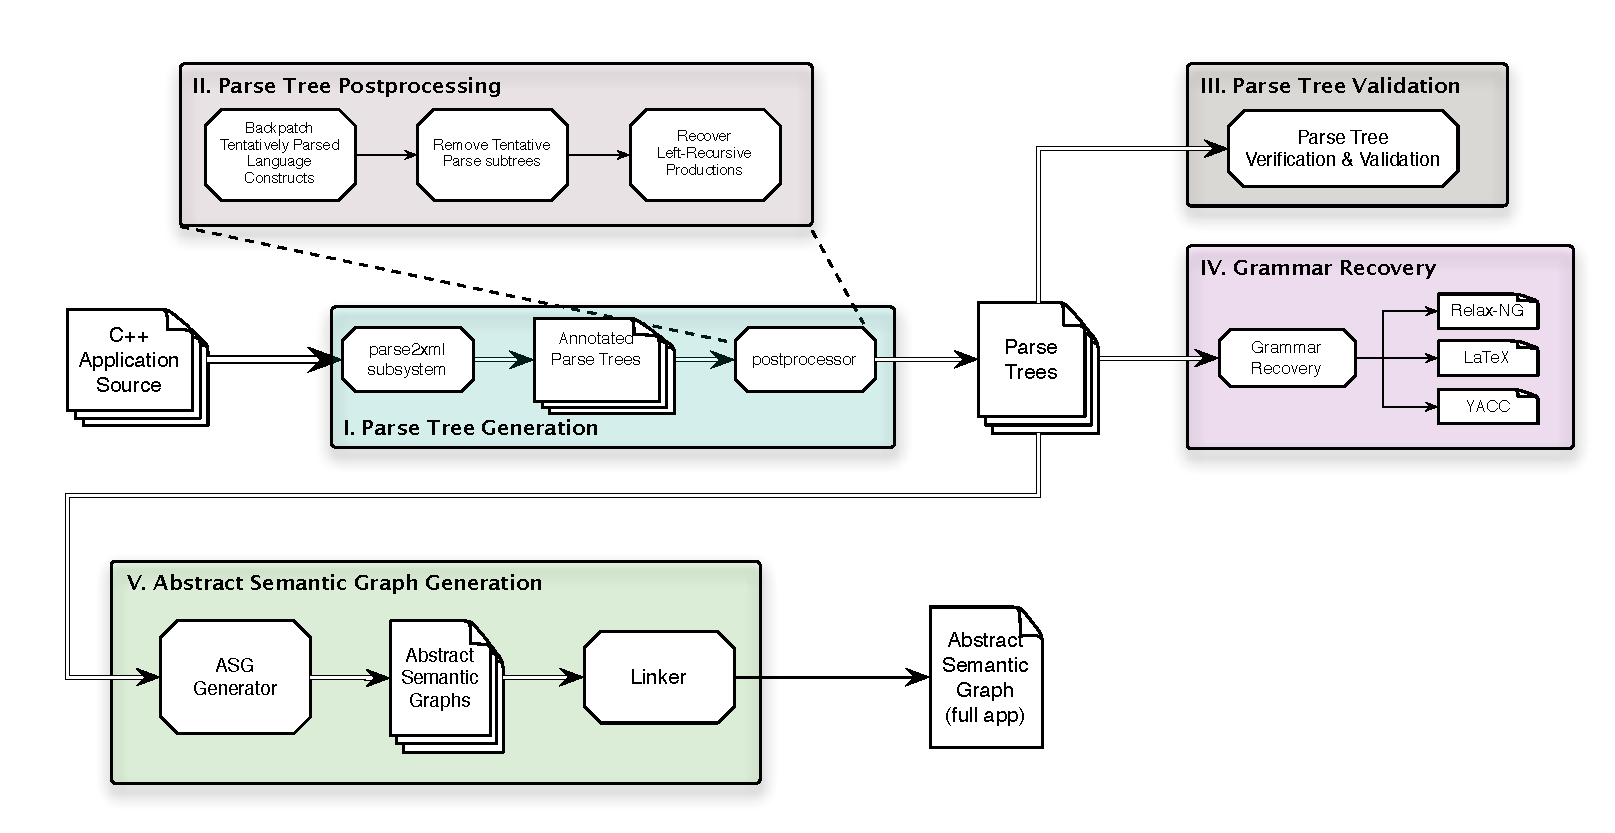
\includegraphics[scale=0.65]{figures/overview_acmse}}
\caption{{\bf \large System Summary}. This figure encapsulates the
important modules in the Hylian system.}
\label{fig:overview}
\figline
\end{figure*}


In this section, we describe Hylian, the system that we developed
to empower a researcher or developer to perform statement-level 
analysis of a program written in a gcc dialect of the {\CPP} language.
Figure \ref{fig:overview} is an overview of Hylian, which
consists of three phases: (1) Parse tree extraction and grammar
recovery, (2) development and generation of an ASG, and 
(3) transformation of the ASG.


The first phase is summarized at the top of Figure \ref{fig:overview} 
by the rectangles labeled 
I, {\sf Parse Tree Generation}; 
II, {\sf Parse Tree Postprocessing};
III, {\sf Parse Tree Validation};
and IV, {\sf Grammar Recovery}.
In module I of the first phase, we generate parse trees for each 
compilation unit in the application by augmenting the 
gcc {\CPP} parser with probes whose output generates
an XML representation for each of the respective parse trees.
The $gcc$ parser performs tentative parsing and then
backtracks to recover from incorrectly chosen alternatives. 
Thus, in module II, the parse subtrees that were emitted as part 
of an incorrect alternative are deleted and the committed subtrees 
are written to a file in XML format.
In module III, the generated parse trees are validated.
Validation entails recovery of a grammar for the gcc
{\CPP} grammar, module IV, and then use of the grammar to 
generate a schema, in Relax NG format.

The second phase, generation of an ASG, is summarized by
the two rectangles, V, {\sf Abstract Semantic Graph generation},
and VI, {\sf ASG verification}, are summarized in the middle
of Figure \ref{fig:overview}.
The focus of this paper is ASG generation, and this will
be described in more detail in Section \ref{sec:method}.


There are many advantages attached to the use of a language-complete
system, such as Hylian, the language-complete ASG 
construction system that we describe,
One of these is the subsequent feasibility of statement 
level transformations and 
subsequent code generation of the transformed ASG.
In reference \cite{IJSEKE},
We show that the use of parse trees does not provide sufficient
information to fully automate the process of generating interface
protocols for the classes in a library and that using the 
language-complete Hylian ASG, the process can be fully automated and, 
in fact, there are even more benefits of using a Hylian ASG.
However, a full explanation of these additional features is
beyond the scope of this paper.




\section{Construction of the ASG}
\label{sec:method}


In this section, we provide an overview of the second phase of
the construction of ASGs, illustrated in the middle of 
Figure \ref{fig:overview} by the rectangles labeled V.
We first describe the problems in building an ASG for the
{\CPP} language and then we describe the procedure we use
in Hylian to construct a language-complete ASG.


\begin{figure*}[htbp]
\centerline{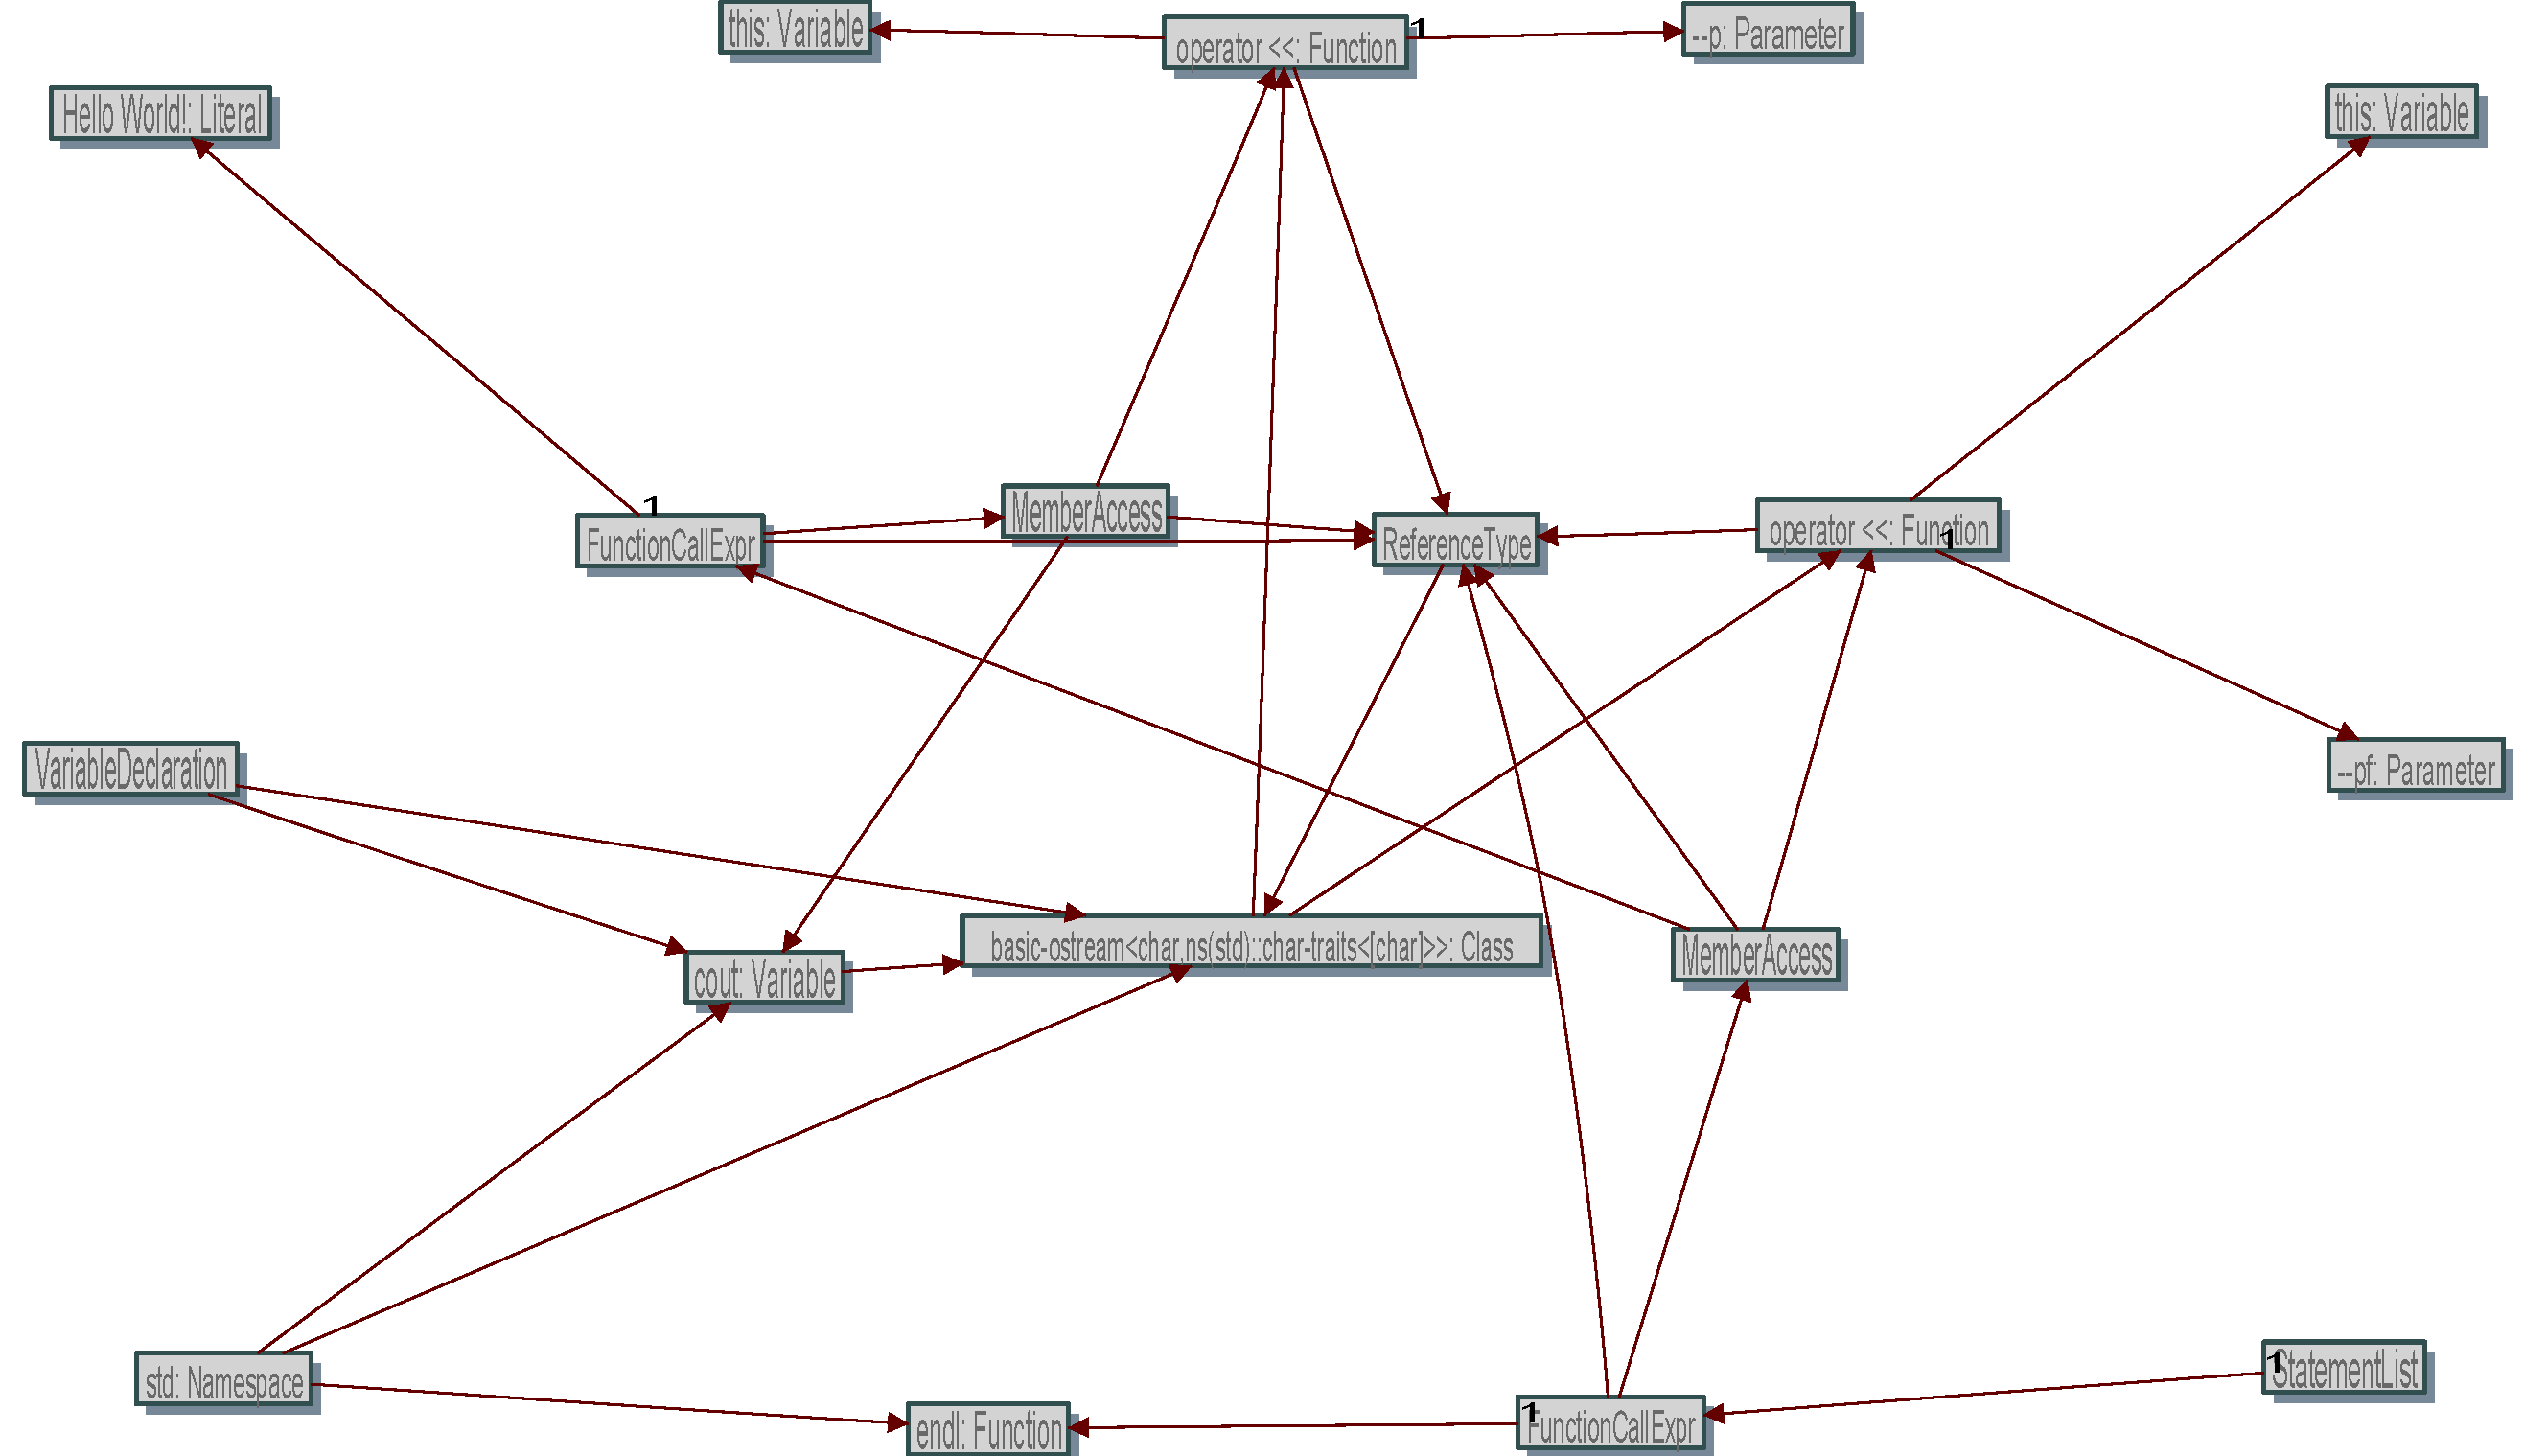
\includegraphics[scale=0.40]{figures/cpphello_full}}
\caption{A language-complete Abstract Semantic Graph for 
a \textsf{Hello World} program}
\label{fig:fullhello}
\figline
\end{figure*}


The attachment of type information to the names used in an
application is fairly straightforward if the program is written
in a procedural language such as C or Fortran. However, 
attaching semantic information to names used in applications
written in a multi-paradigm, composite 
language \cite{Stroustrup1994,dennythesis09}, 
such as {\CPP}, present unique challenges.
These features include data hiding, generics, multiple inheritance
and other constructs that make the attachment of semantic information
much more difficult than in the processing of procedural languages. 
These challenges comprise the bulk of the effort required for
the construction of the Hylian analysis system.

The most imposing of these challenges, name lookup, actually sounds 
uniquely trivial, yet a solution to this problem entails resolving
type information for virtually every production in the {\CPP} grammar.
Thus, name lookup is difficult firstly because of the breadth of
the problem, since the {\CPP} grammar is one of the largest grammars
in use, yet more importantly, is the most complex 
grammar \cite{Power-Malloy:04}.
For example, the {\sf impurity} metric applied to the {\CPP}
grammar shows that, at 85\%, the {\CPP} grammar contains a considerable
density in the edges in the closure of the call graph, especially
compared to the grammars for C, Java and C\#.
The {\sf impurity} metric, together with the application of McCabe's
metric to the {\CPP} grammar, provide further evidence of the
complexity, and the tight coupling of the {\CPP} grammar
productions \cite{Power-Malloy:04}.


As an illustrative example of the issues involved in name lookup
in {\CPP}, consider resolution of the simple three-operand expression 
for printing ``Hello World:''\\ 
\verb++\textsf{\textbf{int} main() \{ std::cout $\ll$ ``Hello, World!'' $\ll$ std::endl; \} }\\
The first operand is \textsf{std::cout} and its type is
{\sf std::ba\-sic\-\_ostream\-$<$char$>$}. The second operand,
a string literal, is type {\sf \textbf{const char}$\ast$}.
Resolving the correct implementation of \textsf{\textbf{operator}$\ll$}
involves examining seventeen methods of the instantiation of
\textsf{std::ba\-sic\_o\-stream}, and five function templates in the
\textsf{std} namespace, that accept a \textsf{std::basic\_ostream}
object as its first argument. 
The Hylian ASG construction algorithm compare the parameters 
for the partially-specialized function template in
\textsf{std::ba\-sic\_o\-stream} and find
those that most closely match the types 
of these first two operands.  When found, that function is instantiated,
inserted into the ASG, and the type of the subexpression is
\textsf{std::basic\_ostream}.
The full ASG for a {\sf hello world} program is illustrated 
in Figure \ref{fig:fullhello}.

\begin{figure}[ph]
   \centering
   \scriptsize
   \begin{tabular}{m{.03\textwidth}m{.7\textwidth}}
 ~1 & \verb++\textsf{\textbf{declare} \emph{tag}: XML tag} \\
 ~2 & \verb++\textsf{\textbf{declare} \emph{syntaxStack}: stack} \\
 ~3 & \verb++\textsf{\textbf{declare} \emph{semanticStack}: stack } \\
 ~4 & \verb++\textsf{\textbf{declare} \emph{parsetreeBuffer}: dictionary} \\
 ~5 & \verb++\textsf{\textbf{declare} \emph{currentParsetreeBuffer}: string} \\
 ~6 & \verb++\textsf{\textbf{declare} \emph{isBuffering}: boolean} \\
 ~7 & \verb++\textsf{\textbf{declare} \emph{currentTemplateDecl}: template declaration} \\
 ~8 & \\
 ~9 & \verb++\textsf{push an empty list onto \emph{semanticStack} and \emph{syntaxStack} } \\
 10 & \verb++\textsf{\emph{tag} $\leftarrow$ getTag()} \\
 11 & \verb++\textsf{\textbf{while} ( more tags in XML Parse Tree ) :} \\
 12 & \verb+  +\textsf{\textbf{if} (\emph{tag} \textbf{is} startTag) :} \\
 13 & \verb+    +\textsf{\textbf{if} ( \emph{tag} \textbf{is} template declaration \textbf{and not} \emph{isBuffering} ) :} \\
 14 & \verb+      +\textsf{\emph{currentParsetreeBuffer} $\leftarrow$ empty parse tree} \\
 15 & \verb+      +\textsf{\emph{currentTemplateDecl} $\leftarrow$ \emph{NULL}} \\
 16 & \verb+      +\textsf{\emph{isBuffering} $\leftarrow$ \emph{TRUE}} \\
 17 & \verb+    +\textsf{\textbf{if} ( \emph{isBuffering} ) :} \\
 18 & \verb+      +\textsf{\textbf{store} \emph{tag} \textbf{in} \emph{currentParsetreeBuffer}} \\
 19 & \verb+      +\textsf{\textbf{if} (\emph{currentTemplateDecl} \textbf{is not} \emph{NULL}) : } \\
 20 & \verb+        +\textsf{\textbf{continue} at top of while } \\
 21 & \verb+    +\textsf{\textbf{append} \emph{tag} to list at top of \emph{syntaxStack} } \\
 22 & \verb+    +\textsf{\textbf{if} ( \emph{tag} \textbf{is} tokenTag ) :} \\
 25 & \verb+      +\textsf{// keyword, constant, symbol, or identifier} \\
 26 & \verb+      +\textsf{\textbf{if} ( \emph{tag} is literal ) :} \\
 27 & \verb+        +\textsf{\textbf{determine} representation and type} \\
 28 & \verb+        +\textsf{\textbf{append} value of literal to list at top of \emph{semanticStack}} \\
 29 & \verb+      +\textsf{\textbf{else if} ( \emph{tag} \textbf{is} name ) :} \\
 30 & \verb+        +\textsf{\textbf{if} ( \emph{tag} \textbf{is} keyword ) :} \\
 31 & \verb+          +\textsf{\textbf{replace} `token' with actual keyword in list at top of} \\
 32 & \verb+             +\textsf{\emph{syntaxStack} (e.g., class)} \\
 33 & \verb+          +\textsf{\textbf{append} \emph{NULL} to list at top of \emph{semanticStack}} \\
 34 & \verb+        +\textsf{\textbf{else} :} \\
 35 & \verb+          +\textsf{\textbf{push} identifier onto list at top of \emph{semanticStack}} \\
 36 & \verb+      +\textsf{\textbf{else if} ( \emph{tag} is symbolTag ) :} \\
 37 & \verb+        +\textsf{\textbf{replace} `token' with symbol value (e.g., replace with `+')} \\
 38 & \verb+        +\textsf{\textbf{append} \emph{NULL} to list at top of \emph{semanticStack}} \\
 39 & \verb+    +\textsf{\textbf{else} :} \\
 40 & \verb+      +\textsf{\textbf{append} \emph{NULL} to list at top of \emph{semanticStack}} \\
 41 & \verb+  +\textsf{\textbf{else if} ( \emph{tag} \textbf{is} endTag ) :} \\
 42 & \verb+    +\textsf{\textbf{if} ( \emph{isBuffering} ) :} \\
 43 & \verb+      +\textsf{\textbf{store} \emph{tag} in \emph{currentParsetreeBuffer}} \\
 44 & \verb+    +\textsf{\textbf{if} (\textbf{not} \emph{isBuffering} \textbf{xor} \emph{currentTemplateDecl} \textbf{is not} \emph{NULL}) :} \\
 45 & \verb+      +\textsf{\textbf{call} function to perform semantic-action on\_tag\_name} \\
 46 & \verb+        +\textsf{i.e., for the tag "$<$/class\_head$>$" call on\_class\_head()} \\
 47 & \verb+      +\textsf{\textbf{pop} \emph{syntaxStack}} \\
 48 & \verb+      +\textsf{\textbf{pop} \emph{semanticStack}} \\
 49 & \verb+      +\textsf{\textbf{replace} \emph{NULL} in list at top of \emph{semanticStack} with result of} \\
 50 & \verb+        +\textsf{semantic-action, i.e. the semantic value of the production} \\
 51 & \\
 52 & \verb+    +\textsf{\textbf{if} (\emph{isBuffering} \textbf{and} \emph{currentTemplateDecl} \textbf{is not} \emph{NULL}) :} \\
 53 & \verb+      +\textsf{\textbf{add} to \emph{parsetreeBuffer}, where the key is the declaration, and the} \\
 54 & \verb+        +\textsf{value is the partially created buffer (in progress).} \\
 55 & \verb+    +\textsf{\textbf{if} (matching close of template\_declaration that started buffering) :} \\
 56  & \verb+       +\textsf{\emph{isBuffering} $\leftarrow$ \emph{FALSE}} \\
 57 & \verb+  +\textsf{\emph{tag} $\leftarrow$ getTag()} \\
   \end{tabular}
\caption{The algorithm used to convert a parse tree into a bottom-up style parse}
\label{fig:asgcons}
\shortline
\end{figure}

\subsection{Parsing parse trees expressed in XML}

The algorithm in Figure \ref{fig:asgcons} parses the XML representation of the parse-tree 
of the original user application code.  The parse-tree parser is a 
top-down SAX XML parser, but we prefer to handle the grammar productions
in bottom-up fashion. 
Thus, to simulate a bottom-up parse we must buffer the XML tags
that represent terminals and non-terminals from the original user
application code, and delay the semantic actions until a complete
sentence encountered.
The semantic action for each production is handled by a function
that accepts two lists: (1) a list of the syntax symbols, and (2)
a list of their corresponding semantic values.  The return value of
the semantic action function is the semantic value of that production.

To correctly handle template classes and functions, we delay total evaluation
of their subtree until we encounter a use later in the parse tree.
When a template definition is encountered, we must parse enough of its
tree to determine its declaration all the while buffering the entire subtree
for later use.  Once we determine the declaration, we stop handling semantic
actions until the matching close tag for the template declaration is reached.
We then store the template declaration and its corresponding parse tree
in a dictionary until a usage of the template requires instantiation.


%A summary of the actions required to build an ASG from an XML representation
%of a parse tree for a compilation unit is listed in Figure \ref{fig:asgcons}.
%The parse tree is result of the first phase of our system shown in 
%Figure \ref{fig:overview}.

\subsection{Overview of ASG construction}

To generate an ASG, we first prune 
the generated parse trees to eliminate unnecessary
non-terminals and empty productions. We then annotate the
pruned parse tree with semantic information, such as the type
or scope of a variable. In the case of templates, we must
build an ASG representation of the instantiated template.
After we have extended each of the parse trees with semantic
information to produce an ASG for each compilation unit,
we then {\em link}, or merge, the ASGs into a single
ASG for the entire program.
Exposition of the full algorithm for ASG construction is
beyond the scope of this paper. In this section,
we provide an overview of this construction  process.
The interested reader may consult reference \cite{duffythesis}
for details, and an algorithm, for ASG construction.


The algorithm for ASG construction uses seven data structures and a while
loop that examines each XML tag in turn. 
The first data structure, {\sf tag}, is the current XML tag.
The next two data structures facilitate a bottom up parse using
the tags from the top-down XML parser:
{\sf syntaxStack}, a stack of lists that contain terminals and
non-terminals encountered in the bottom-up parse;
and {\sf semanticStack}, a stack of lists that contain semantic values
encountered in the bottom up parse of the parse tree.
The final four data structures facilitate template declaration buffering
and instantiation:
{\sf parsetreeBuffer}, a dictionary that maps a template declaration
to its respective parse tree;
{\sf currentParsetreeBuffer}, a buffer for a parse tree of a template so
that when a template declaration is encountered the parse action is delayed 
until the template is instantiated and fully defined by its usage;
{\sf isBuffering}, a boolean indicating that the current tag
is the child of a template declaration;
and, finally,
{\sf currentTemplateDecl}, a handle for a declaration that
contains information to facilitate name lookup for the currently buffered
template declaration, which contains scope information, name, 
arguments for the template, and possibly information about parameters
to a function template.


{\protect
\begin{table}[th]
\footnotesize
\centering
\begin{tabular}{|l|r|r|r|}
\hline
 \multicolumn{1}{|}{\bf Graph} &
 \multicolumn{2}{|c|}{\bf Hello World} & 
 \multicolumn{1}{c|}{\bf Game}\\
 & {\bf C} & \textbf{{\CPP}} &  {\bf AlephOne} \\
\hline
\textbf{Parse Trees} & & & \\
No. Compilation Units & 1 & 1 & 176 \\
No. System Terminal & 2,930 & 132,122 & 30,339,853 \\
No. User Terminal & 13 & 16 & 3,441,975 \\
No. Total Terminal & 2,943 & 132,138 & 33,781,828 \\
No. Non-Terminals & 13,404 & 518,788 & 128,818,128 \\
%Max Branch Length   & 223 & 374 & 3,671 \\
%Avg. Branch Length  & 123.47 & 215.33 & 652.71 \\
\hline
\textbf{ASG} & &  & \\
No. Vertices & 984 & 21,861 & 1,914,869 \\
No. Vertices (linked) & & & 478,642 \\
No. Edges & 2,098 & 45,444 & 3,632,959 \\
No. Edges (linked) & & & 1,003,413 \\
No. Statements & 137 & 2,263 & 1,512,638 \\
No. Statements (linked) & & & 115,534 \\
\hline
\end{tabular}
\caption {Statistical results For Hylian}
\label{tab:asgstats}
%\shortline
\shortline
\end{table}

\newpage
\section{Results}
\label{sec:results}




In this section we provide some interesting results for ASGs that 
we have built using Hylian.
Table \ref{tab:asgstats} summarizes these results for three
programs in our test suite: a {\sf Hello World} program written in
C and {\CPP}, and {\sf AlephOne}, a rather large
video game translated into {\CPP} that uses the
Simple Direct Media Layer (SDL) API, as well as the Lua
embedded scripting engine.
There are two sections of data in the table: the top section 
that summarizes results for the construction of {\sf Parse Trees}, 
and the bottom section that summarizes results for the construction
of ASGs. We are comparing parse trees and ASGs in the top and bottom
sections to show the reduction in the size of ASGs compared to parse
trees, and the reduction in size when the ASGs for each compilation 
unit in a program are {\em linked}, or merged,
into a single ASG for the entire program.


To evaluate the results, we first consider the data
for the three ``Hello World'' programs.
The first column in the table describes the information in the particular
row of the table, and the next three columns represent information
for the ``Hello World'' programs written in C and {\CPP}.
Our first result shows that both the C and {\CPP}
versions of ``Hello World'' consist of a single {\sf Compilation Unit},
as shown by the first row of data in the table for columns two, three
and four; however, the {\sf No. System Terminals} in the C version has
2,930 terminals in the parse trees, but the {\CPP} versions have 132,122
terminals in their parse trees, so that the {\CPP} version has almost
two orders of magnitude more terminals than the C version. This
differential is caused by the inclusion of {\sf iostream} and much
of the {\CPP} library in the {\CPP} version of ``Hello World.''
Also, the {\sf No. System Terminals} in the {\sf AlephOne} program
is 30,339,853 (first row, last column of the table), 
illustrating the large number of system terminals
needed for a standard video game. The remaining rows at the top
of the Table \ref{tab:asgstats} reflect similar comparisons.

The bottom section of Table \ref{tab:asgstats} summarizes results
for the ASGs that Hylian builds. The second and third columns in
the bottom section compare the ASG for a full parse of a C and
a {\CPP} ``Hello World'' program. For example, the third row of
the bottom section of the table shows that there are 984 vertices
in the C version, and 21,861 vertices in the {\CPP} version, an
order of magnitude increase. Since there is only one compilation
unit in each ``Hello World'' program, there are is only one ASG
and therefore no vertices are linked; thus, the second and fourth
rows in the bottom section of the table do not list any values
for {\sf No. Vertices (linked)} or {\sf No. Edges (linked)}.




\section{Conluding Remarks}
\label{sec:conclude}


In this paper, we described Hylian, a system for construction
of a language-complete ASG that provides statement-level
analysis, both static and dynamic, of a {\CPP} application.
We performed various verification and validation metrics to the ASG,
including a viewer that can visualize any graph in GXL format,
to provide assurance for a developer that the ASGs that Hylian builds
correctly represent the program under investigation.
To evaluate space considerations for Hylian ASGs, we have
provided some results that describe the size of the generated
ASGs.  Our future work entails using the Hylian system to
perform transformations on the ASG, and generate {\CPP}
code for the transformed ASG.




\bibliographystyle{abbrv}
\bibliography{bib/paper}

\end{document}

